% Paired illustration of the same inspected C12/C10 development cases.
\documentclass[tikz,border=2pt]{standalone}
\usepackage{fontspec}
\setsansfont{Arial}
\usetikzlibrary{arrows.meta}
\definecolor{blue}{HTML}{0072B2}
\definecolor{orange}{HTML}{B36B00}
\definecolor{ink}{HTML}{303843}
\begin{document}
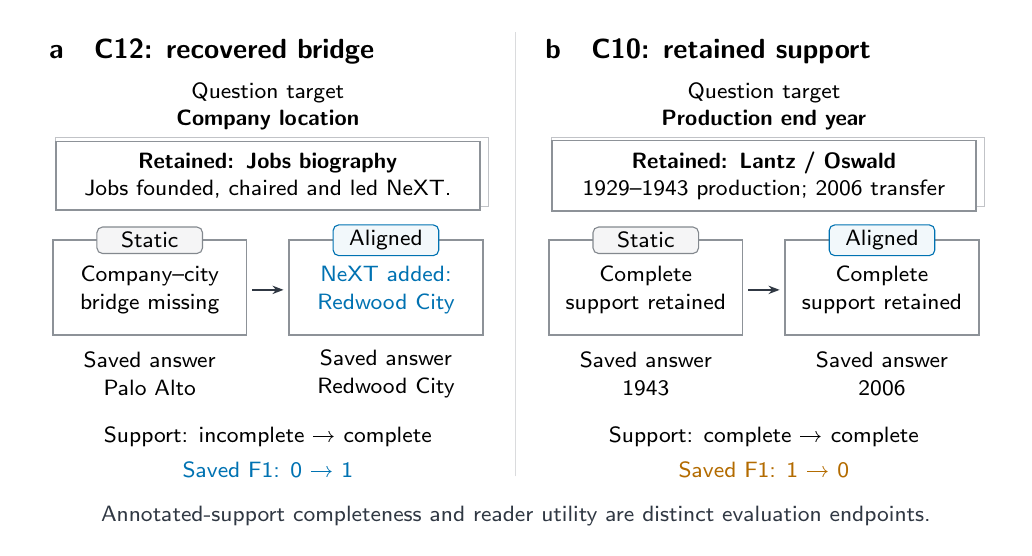
\begin{tikzpicture}[x=1cm,y=1cm,font=\sffamily\fontsize{8.5}{10}\selectfont,
 head/.style={font=\sffamily\bfseries\fontsize{10}{11}\selectfont,anchor=west},
 doc/.style={draw=ink!55,fill=white,line width=.6pt,inner sep=4pt,align=center},
 badge/.style={draw=ink!60,fill=ink!5,rounded corners=2pt,text width=1.2cm,align=center,inner sep=2pt},
 flow/.style={-{Stealth[length=4pt]},draw=ink,line width=.7pt}]
\path[use as bounding box] (0,0) rectangle (12.4,6.35);
\draw[ink!18] (6.2,.65)--(6.2,6.3);
\node[head] at (.15,6.05) {a\quad C12: recovered bridge};
\node[head] at (6.45,6.05) {b\quad C10: retained support};
\node[align=center] at (3.05,5.35) {Question target\\\textbf{Company location}};
\node[align=center] at (9.35,5.35) {Question target\\\textbf{Production end year}};
% Offset source cards summarize evidence retained in both contexts.
\foreach \x in {.35,6.65} {
 \draw[ink!30,fill=white] (\x,4.08) rectangle +(5.5,.87);
}
\node[doc,text width=5.1cm,minimum height=.87cm] at (3.05,4.47)
 {\textbf{Retained: Jobs biography}\\Jobs founded, chaired and led NeXT.};
\node[doc,text width=5.1cm,minimum height=.87cm] at (9.35,4.47)
 {\textbf{Retained: Lantz / Oswald}\\1929--1943 production; 2006 transfer};
% Identical cards, badges, baselines and spacing in both panels.
\foreach \x in {1.55,4.55,7.85,10.85} {
 \draw[ink!55,fill=white,line width=.6pt] (\x-1.23,2.45) rectangle (\x+1.23,3.65);
}
\foreach \x in {1.55,7.85} \node[badge] at (\x,3.65) {Static};
\foreach \x in {4.55,10.85} \node[badge,draw=blue,fill=blue!5] at (\x,3.65) {Aligned};
\node[align=center,text width=2.25cm] at (1.55,3.02) {Company--city\\bridge missing};
\node[align=center,text width=2.25cm,text=blue] at (4.55,3.02) {NeXT added:\\Redwood City};
\node[align=center,text width=2.25cm] at (7.85,3.02) {Complete\\support retained};
\node[align=center,text width=2.25cm] at (10.85,3.02) {Complete\\support retained};
\draw[flow] (2.85,3.02)--(3.25,3.02);
\draw[flow] (9.15,3.02)--(9.55,3.02);
\foreach \x/\answer in {1.55/Palo Alto,4.55/Redwood City,7.85/1943,10.85/2006}
 \node[align=center] at (\x,1.95) {Saved answer\\\answer};
\node[align=center] at (3.05,1.15) {Support: incomplete → complete};
\node[align=center] at (9.35,1.15) {Support: complete → complete};
\node[align=center,text=blue] at (3.05,.73) {Saved F1: 0 → 1};
\node[align=center,text=orange] at (9.35,.73) {Saved F1: 1 → 0};
\node[align=center,text=ink] at (6.2,.15)
 {Annotated-support completeness and reader utility are distinct evaluation endpoints.};
\end{tikzpicture}
\end{document}
